% digitalizace https://yangcha.github.io/iview/iview.html
%
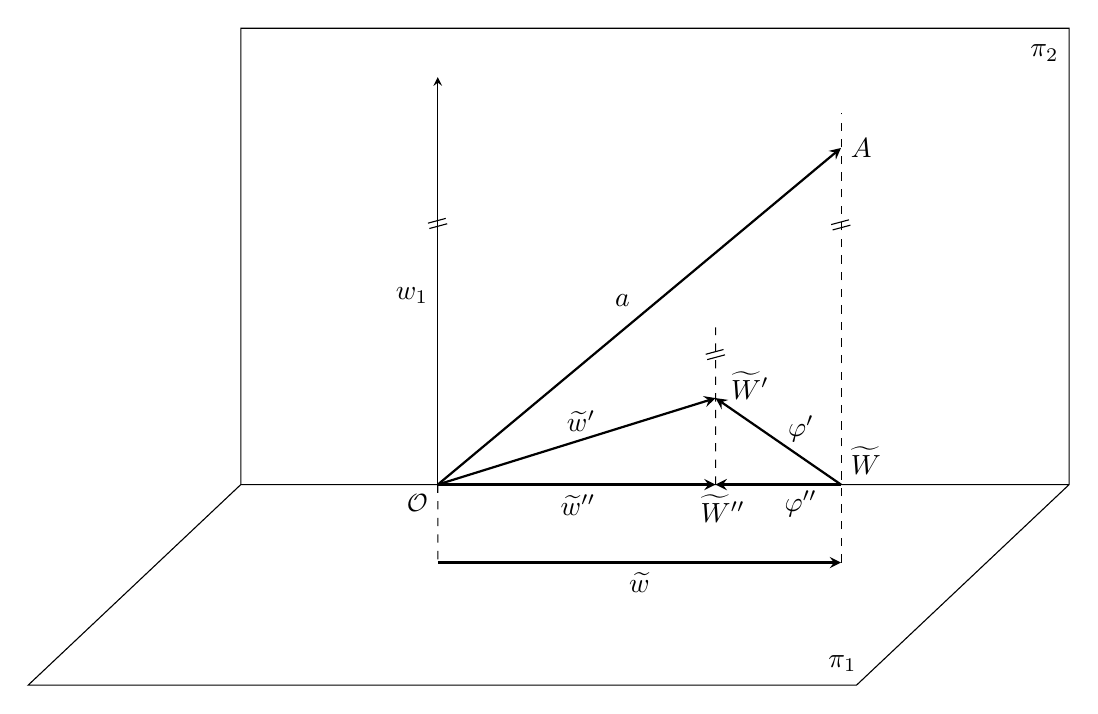
\begin{tikzpicture}[xscale=9,yscale=-9,>=stealth]

  \begin{scope}   % projekcni roviny pi_1 a pi_2

    \def\Mx{0.331};
    \def\My{0.684};
    \coordinate(M) at (\Mx,\My);
    \def\Nx{1.500};
    \def\Ny{\My};
    \coordinate(N) at (\Nx,\Ny);
    \def\Px{\Nx};
    \def\Py{0.040};
    \coordinate(P) at (\Px,\Py);
    \def\Rx{\Mx-0.300};
    \def\Ry{0.967};
    \coordinate(R) at (\Rx,\Ry);
    \def\Qx{\Mx};
    \def\Qy{\Py};
    \coordinate(Q) at (\Qx,\Qy);
    \def\Sx{\Nx-0.300};
    \def\Sy{\Ry};
    \coordinate(S) at (\Sx,\Sy);

    \def\Ty{0.110};   % odsazeni vektoru \widetilde w pod osou O-B

    \draw[thin] (M)--(N)--(P)--(Q)--(M)--(R)--(S)--(N);

    \node at (\Px - 0.035,\Py + 0.035) {$\pi_2$};
    \node at (\Sx - 0.020,\Sy - 0.030) {$\pi_1$};

    \def\Ox{0.609};
    \def\Oy{\My};
    \coordinate (O) at (\Ox,\Oy);
    \node at (O) [below left] {{\small $\mathcal{O}$}};

    \def\Ax{1.178};
    \def\Ay{0.209};
    \coordinate (A) at (\Ax,\Ay);
    \def\Bx{\Ax};
    \def\By{\My};
    \coordinate (B) at (\Bx,\By);
    \def\Cx{1.001};
    %%%\def\Cy{0.775};   obr 6.1
    \def\Cy{\Oy};
    \coordinate (C) at (\Cx,\Cy);
    \def\Dx{\Cx};
    \def\Dy{0.562};
    \coordinate (D) at (\Dx,\Dy);

    \def\Ex{\Ox};
    \def\Ey{\Ay-0.100};
    \coordinate (E) at (\Ex,\Ey);
    \draw[ ->] (O)--(E);
    \node at (\Ex,0.417) [left] {$w_1$};
    \node at (\Ex,0.317) {\rotatebox{15}{$\overline{\overline{~~}}$}};

    \draw[thick, ->] (O)--(A);
    %%%\draw[thick, ->] (O)--(B);   obr 6.1
    \draw[thick, ->] (O)--(C);
    \draw[thick, ->] (O)--(D);
    \draw[thick, ->] (B)--(C);
    \draw[thick, ->] (B)--(D);

    \node at (A) [right] {$A$};

    \draw[thin, dashed] (\Bx,\By+\Ty)--(\Ax,\Ay-0.050);
    \node at (\Ax,\Ay+0.110) {\rotatebox{15}{$\overline{\overline{~~}}$}};
    \draw[thin, dashed] (C)--(\Dx,\Dy-0.100);
    \node at (\Dx,\Dy-0.060) {\rotatebox{15}{$\overline{\overline{~~}}$}};

    \node[above left ] at ({(\Ox+\Ax)/2},{(\Oy+\Ay)/2}) {$a$};
    \node[above right] at (B) {$\widetilde W$};
    \node[below right] at ({(\Bx+\Cx)/2-0.005},{(\By+\Cy)/2-0.005})
         {$\varphi''$};
    \node[below] at (\Cx+0.010,\Cy) {$\widetilde W''$};
    \node[below left ] at({(\Ox+\Cx)/2+0.040},{(\Oy+\Cy)/2})
         {$\widetilde w''$};
    \node[above left ] at({(\Ox+\Dx)/2+0.040},{(\Oy+\Dy)/2})
         {$\widetilde w'$};
    \node[above right] at({\Dx+0.008},{\Dy+0.015}) {$\widetilde W'$};
    \node[below right] at ({(\Bx+\Dx)/2},{(\By+\Dy)/2-0.050})
         {$\varphi'$};

     %%%\clip (O)--(C)--(B)--(D)--cycle;    obr 6.1
     %%%\foreach \i in {0,...,30}
     %%%{
     %%%   \def\dx{0.02*\i};
     %%%   \draw[ultra thin] (\Ox + \dx,\Cy+0.1)--(\Ox + \dx,\Dy-0.2);
     %%%}

    \draw[dashed] (O)--(\Ox,\Oy+\Ty);
    \draw[thick, ->] (\Ox,{\Oy+\Ty})--(\Bx,\By+\Ty);
    \node[below] at ({(\Ox+\Bx)/2},{\Oy+\Ty}) {$\widetilde w$};

  \end{scope}

\end{tikzpicture}

%
